\chapter{Conclusion and ongoing work}
\label{cha:conclusion}

Here, we would like to revisit the thesis statement before setting directions for ongoing/future work.

\begin{tcolorbox}[width=\textwidth]
Context-guided attention improves multi-modal content understanding at diverse scales.
\end{tcolorbox}


Till now, we have developed models based on context-guided attention for macro/instance level content understanding tasks w.r.t. domains of movies, TV shows, natural scenes, and advertisements. The content understanding tasks are reliant on the representations learned through context-guided attention mechanisms. Here, we would like to pose the following question regarding the enhancement of these learned representations:

\begin{itshape}
Q: Can we guide the representations learned through context-guided attention to be optimal yet robust for the given macro/instance level task?
\label{context:macro instance level}
\end{itshape}

In terms of guidance, we would like to consider the available knowledge from pretrained multimodal models. With the increase in web-based data sources, there is a trend toward the curation of large-scale weakly aligned datasets consisting of images/videos and noisy descriptions like LAION-5B \cite{schuhmann2022laionb}, CC-12M \cite{changpinyo2021cc12m}, WebVid \cite{Bain21}. The curation of these large-scale sources has led to the rise of multimodal pretraining \cite{wang2022MMPTMSurvey}, where transformer-based models are guided by certain objectives as follows:
\begin{itemize}

  \item \textbf{Image-text matching:} Detect whether the image and text pairs are aligned with each other  
 \item \textbf{Word-region alignment:} Detect whether certain words in the descriptions are matched to image regions
 \item \textbf{Caption generation:} Generate a natural language caption to match the given description with the image
 
\end{itemize}

The aforementioned pretraining tasks are certain examples of objectives used for large-scale models and by no means comprise an exhaustive list. The pretraining stage is followed by subsequent finetuning operations for a wide variety of downstream classification and generative tasks, as mentioned below:

\begin{itemize}

    \item \textbf{Classification tasks:} Visual-question answering, Video-language inference, Visual entailment, Category recognition, Multi-modal sentiment analysis
    \item \textbf{Generative tasks:} Image/Video captioning, Visual dialogue, Multimodal machine translation
    
\end{itemize}
 An outline of the pretraining and finetuning operation is shown in Fig \ref{multimodal pretraining}.

 \begin{figure}[h!]
    \centering
    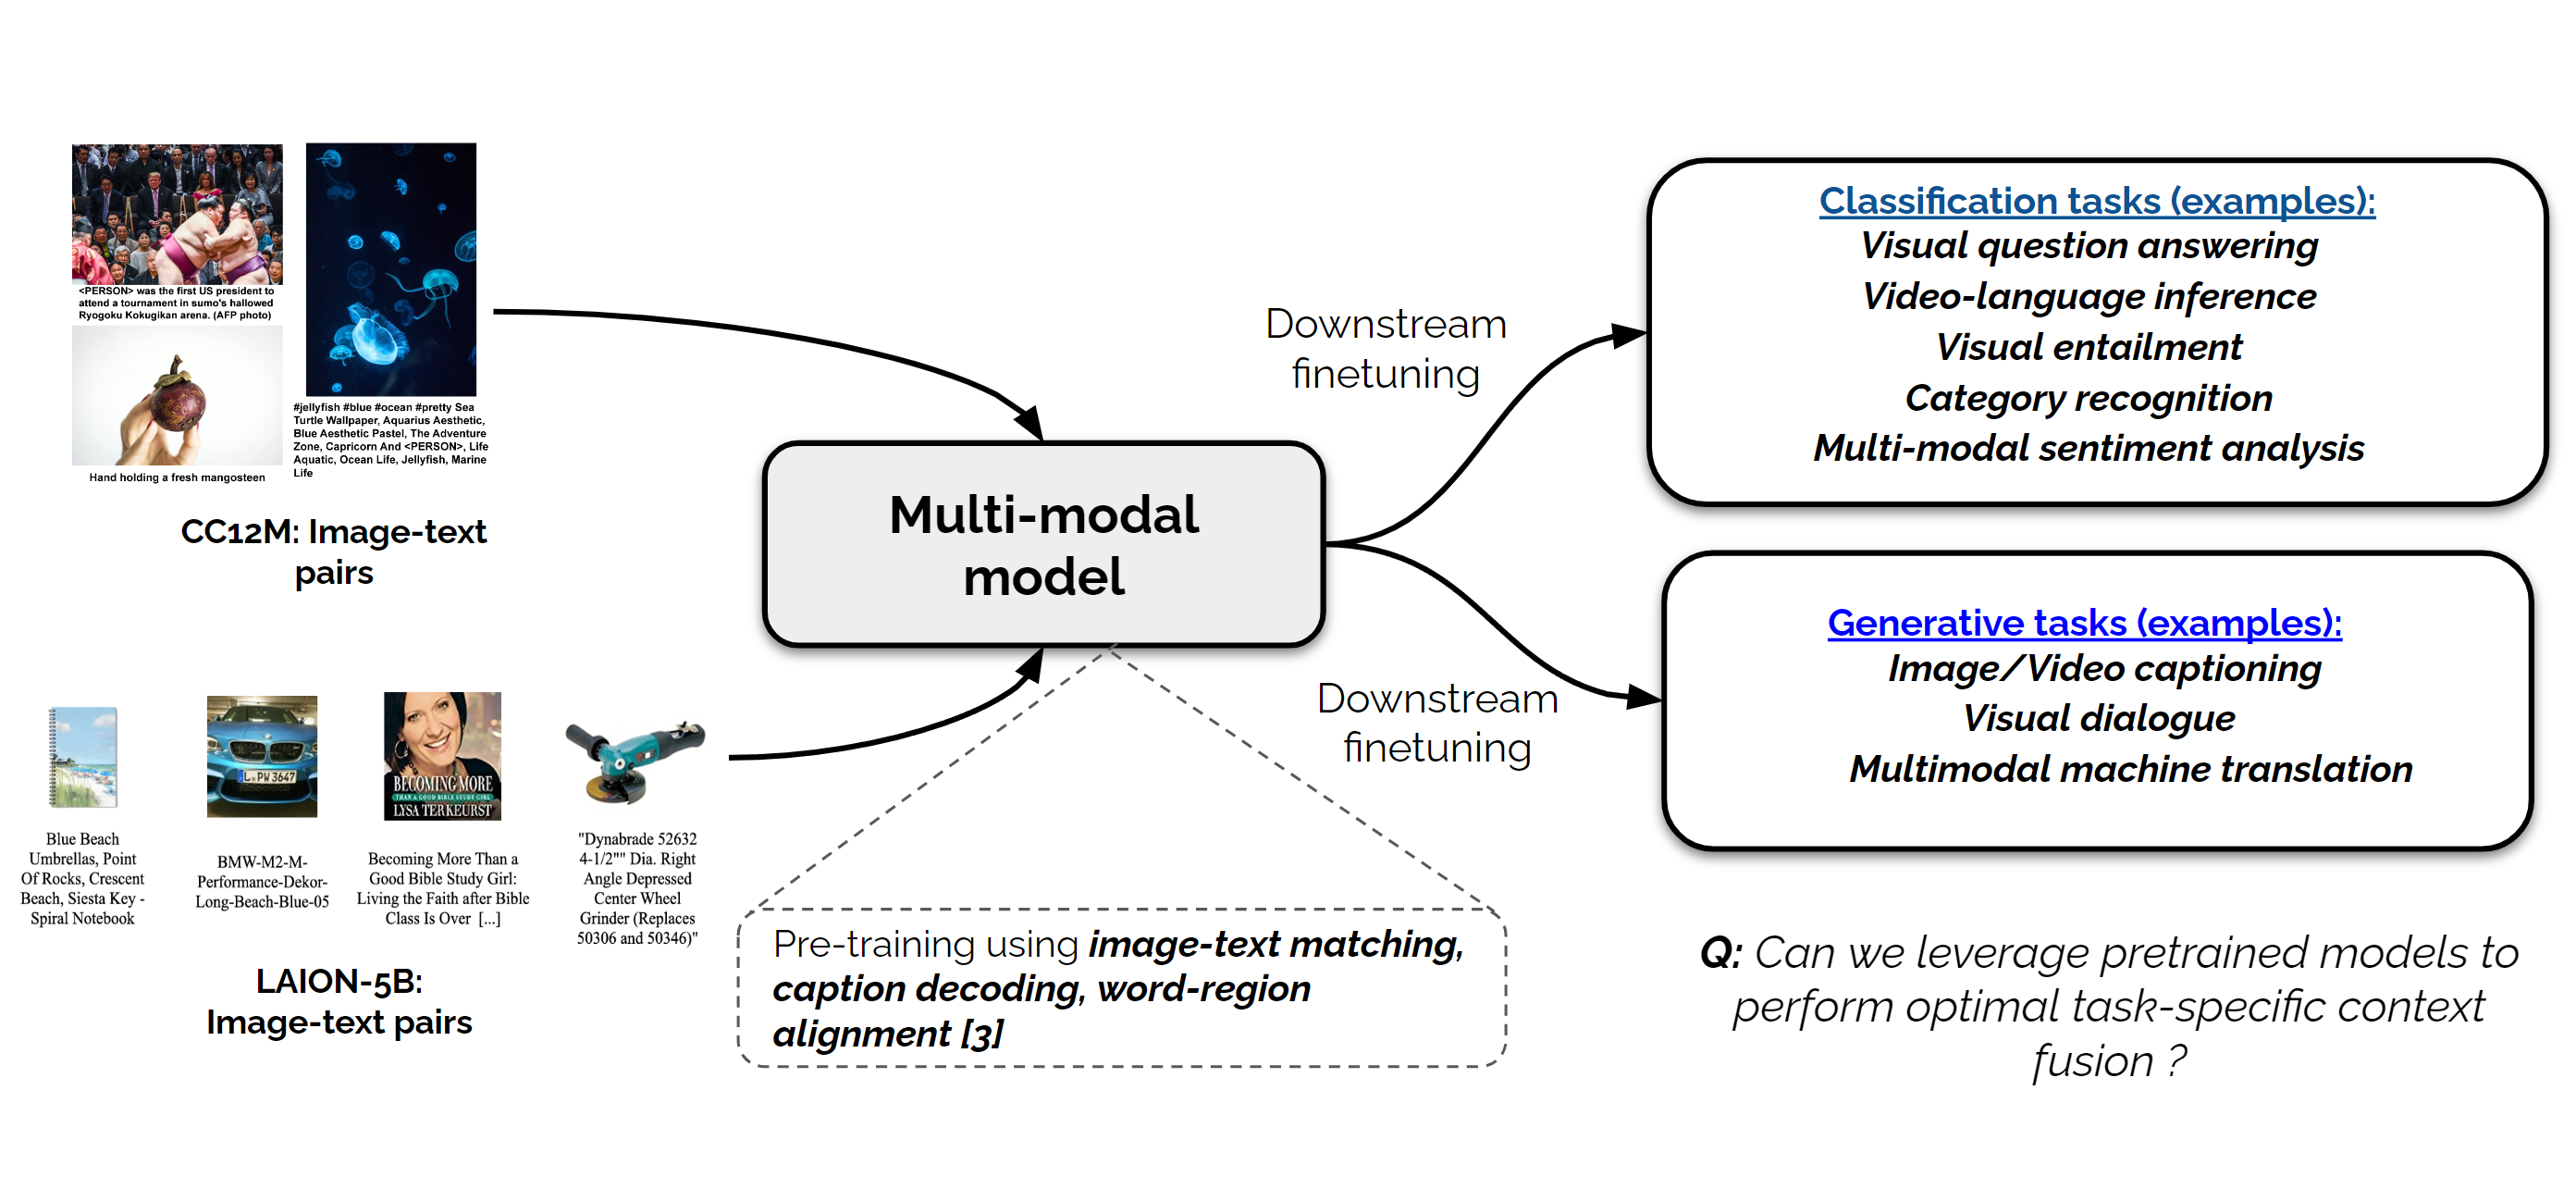
\includegraphics[width=\textwidth]{figures/multimodal_pretraining.png}
    \caption{Pretraining and finetuning operation pipeline in multimodal models.}
    \label{multimodal pretraining}
 \end{figure}

Hence we would like to recast the previous mentioned question to include the role of multimodal pretrained knowledge as follows:

\begin{itshape}
Q: Can we leverage existing large-scale multimodal knowledge to obtain optimal yet robust context-guided representations for given macro/instance-level tasks?
\end{itshape}

With this question, we introduce the concept of Information Bottleneck and how it can be used to obtain optimal yet robust representations for a given task.

\section{Information Bottleneck}

The information bottleneck principle \cite{Tishby2015DeepLA} formulates the goal of deep learning as a trade-off between compression and predictive power. If a given task has associated inputs $X$ and labels $Y$ and the intermediate layer representations of a deep learning model are denoted by $T$, then the optimal task-specific representation can be obtained through the following lagrangian formulation:

\begin{equation}
    L_{IB}= I(Y;T) - \beta I(X;T)
\end{equation}

Here, the objective aims at 
\begin{itemize}
    \item \textbf{Increasing predicting power:} Maximize the mutual information (MI) between labels $Y$ and representations $T$. 
    \item \textbf{Representation compression:} Minimize the mutual information (MI) between inputs $X$ and representations $T$.
\end{itemize}
The parameter $\beta$ controls the relative contributions of the two objective terms. In our case, we would like to explore the usage of information bottleneck as a regularization objective for pretrained multimodal models and its impact on macro and instance-level content understanding tasks under a variety of input settings. We outline our proposed work in the following sections:

\subsection{Related work}
Information Bottleneck (IB) has been utilized for low-resource finetuning of BERT for natural language inference and sentiment analysis tasks in \cite{Mahabadi2021VariationalIB}. Additional usage of information bottleneck includes its usage as task-specific regularizer for learning adversarially robust representations in language models \cite{wang2021infobert}. In the domain of multimodal learning, IB as a regularizer has enabled learning of multimodal representations robust to linguistic variations, image corruptions for visual question answering task \cite{Jiang2022CorrelationIB}. 

\subsection{Information bottleneck and multimodality}

\subsection{Proposed work (A) - Optimal task-specific representations}
\label{Optimal task-specific representations}
In the first part of the proposed work, we would like to benchmark the performance of various multimodal models under the impact of information bottleneck for content understanding tasks. Since finetuning multimodal models is a memory-intensive operation, we would like to explore the parameter settings under which optimal task-specific representations can be extracted after using the information bottleneck as a regularizer. The outline of the proposed work can be found in Fig \ref{optimal_task_representations}.
The context-processing operation extracts contextual information from the given multimodal content through various modalities. The processed contextual information is passed as input to a pretrained multimodal model with a wide variety of parameter settings:
\begin {itemize}
\item \textbf{Linear-Probe:} Finetuning of the task-specific classifier head only and complete freezing of the multimodal encoder.
\item \textbf{Parameter efficient techniques:} Usage of parameter efficient techniques like LoRA, Adapters, prefix tuning for the multimodal encoder
\item \textbf{Full finetuning:} Complete finetuning of the multimodal encoder.
\end{itemize}
For the above parameter settings, we would like to investigate the impact of information bottleneck guidance while finetuning for a host of macro and instance-level tasks as follows:

\begin{itemize}
    \item \textbf{Advertisement video understanding:} Proposed MM-AU Benchmark
    \item \textbf{Hateful content detection:} Hateful memes \cite{Kiela2020TheHM} dataset
    \item \textbf{Movie understanding:}  Movie genre classification \cite{2019Moviescope}, MMIMDB \cite{Arevalo2017GatedMU}
    \item \textbf {Human affect understanding:} Emotic \cite{kostiPAMI}, CAER \cite{CAER-S}
\end{itemize}
\begin{figure}
 \centering 
 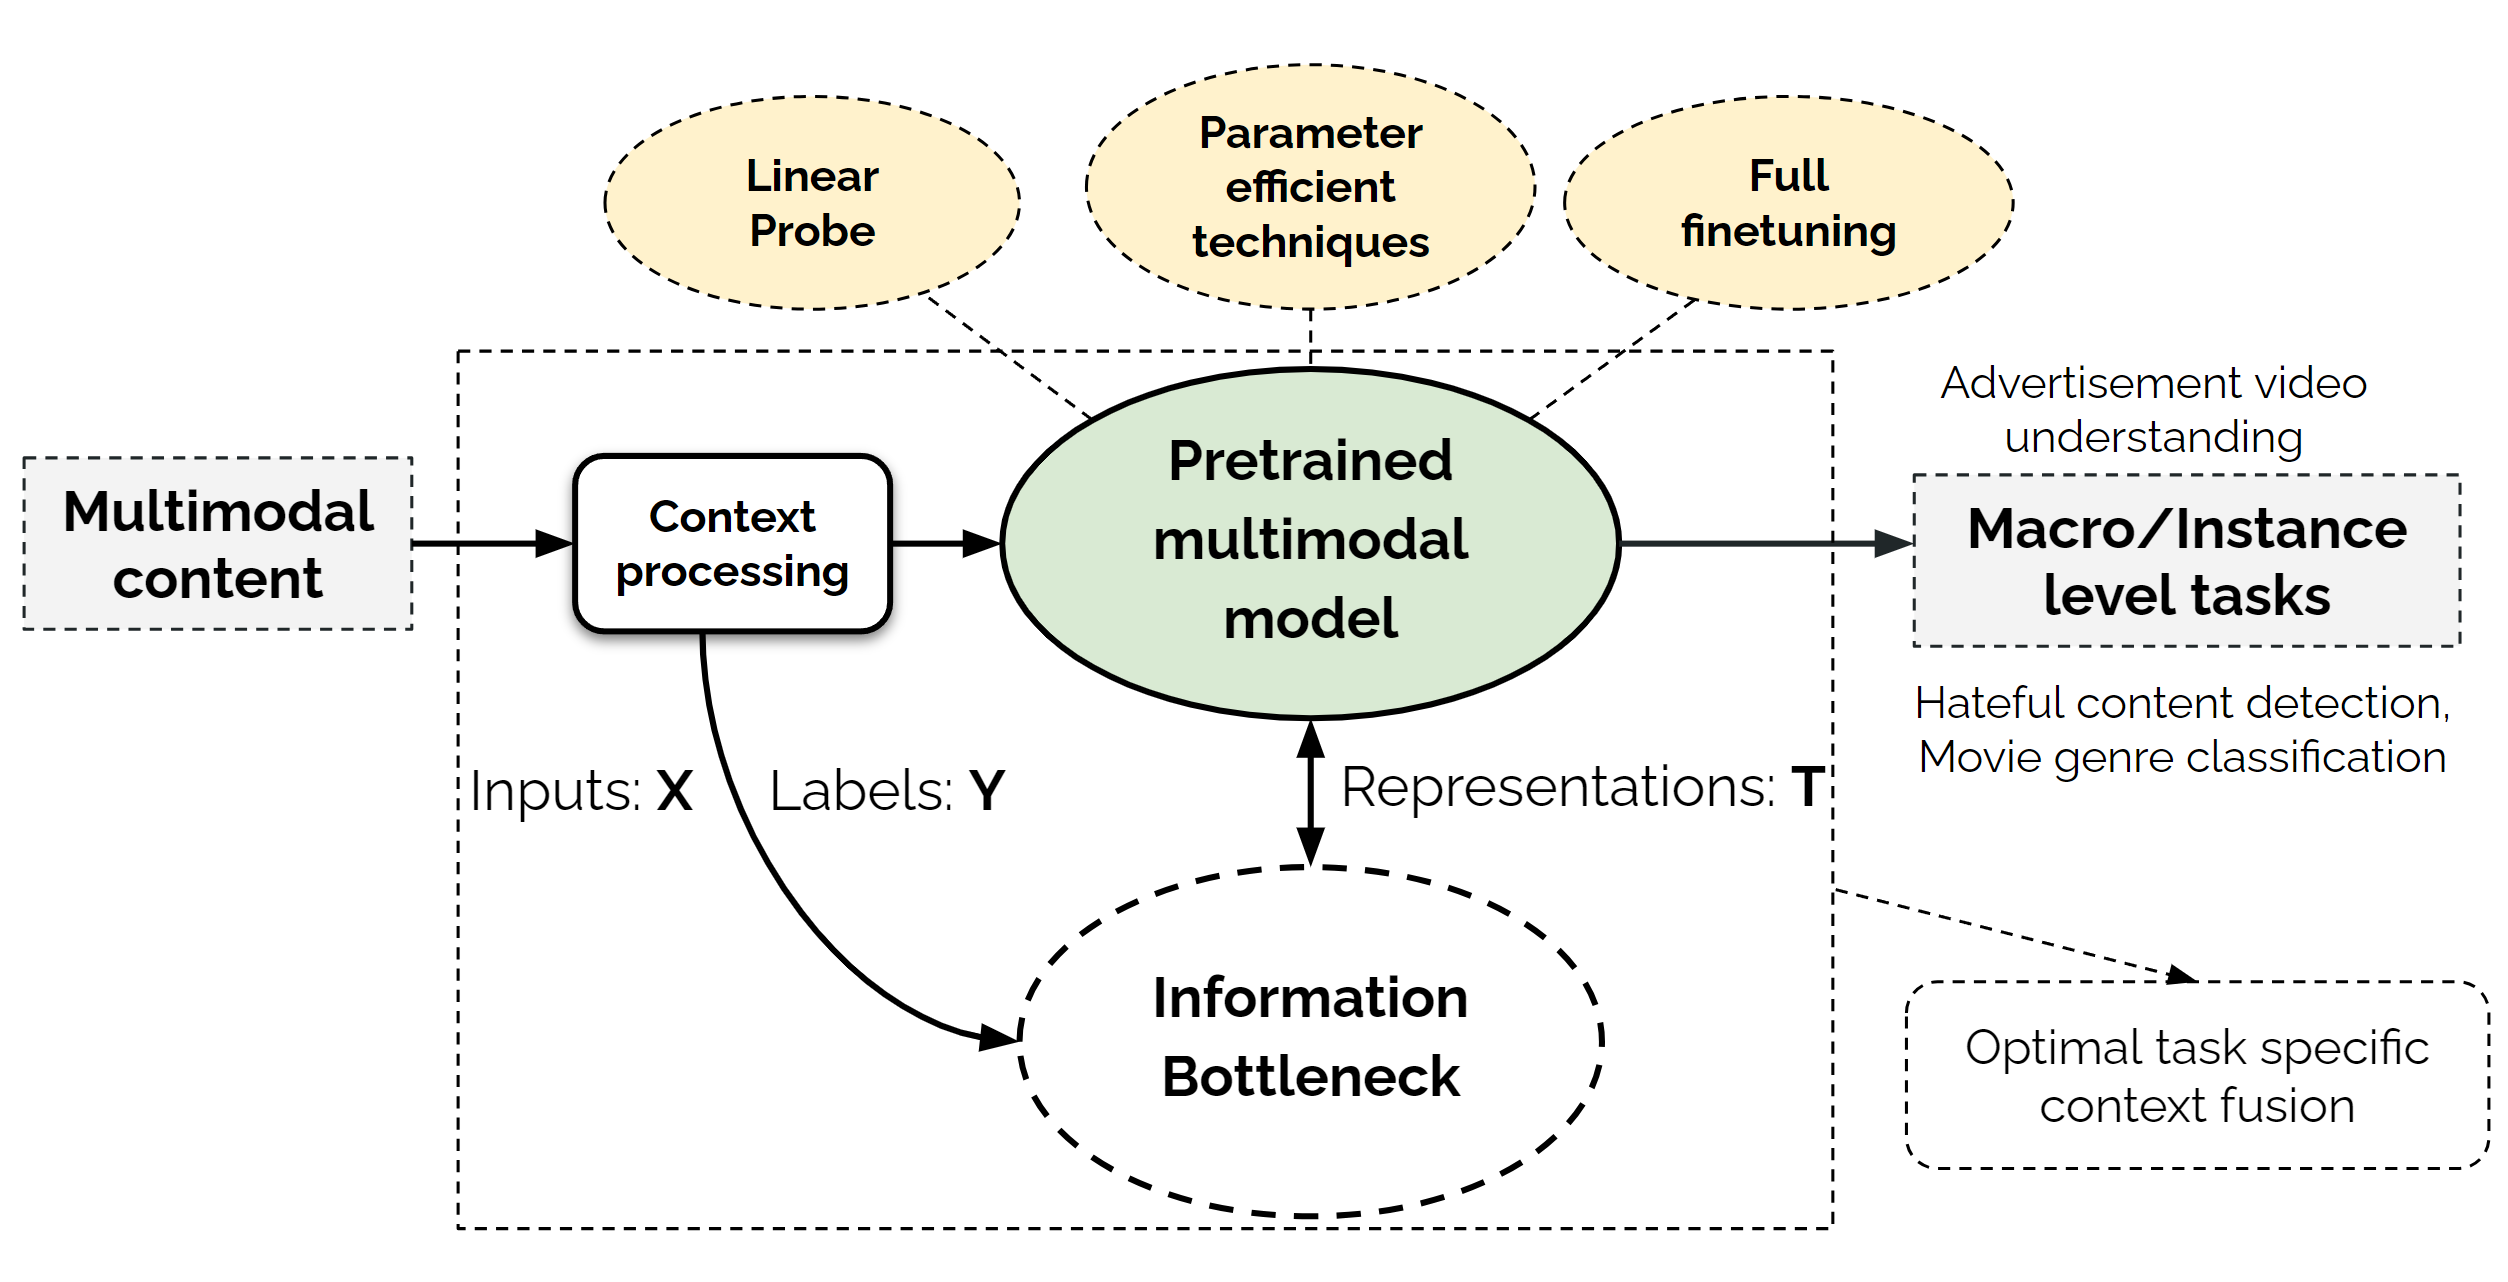
\includegraphics[width=\textwidth]{figures/optimal_task_representations.png}
 \caption{Optimal macro and instance-level task representations based on information bottleneck under different parameter settings}
 \label{optimal_task_representations}
\end{figure}

In terms of architecture, we plan to use the following based on different modality combinations:
\begin{itemize}
\item \textbf{Vision-language:} BLIP-2 \cite{Li2023BLIP2BL}, ViLT \cite{Kim2021ViLTVT}
\item \textbf{Audio-visual:} UAVM model \cite{uavm_gong}
\end{itemize}


\subsection{Proposed work (B) - Characterizing robustness}

